\documentclass[journal,12pt,twocolumn]{IEEEtran}
\usepackage[compact]{titlesec}
\usepackage{setspace}
\usepackage{gensymb}
\singlespacing
\usepackage[cmex10]{amsmath}
\usepackage{amsthm}
\usepackage{mathrsfs}
\usepackage{txfonts}
\usepackage{stfloats}
\usepackage{bm}
\usepackage{cite}
\usepackage{cases}
\usepackage{subfig}
\usepackage{longtable}
\usepackage{multirow}
\usepackage{enumitem}
\usepackage{mathtools}
\usepackage{steinmetz}
\usepackage{tikz}
\usepackage{circuitikz}
\usepackage{verbatim}
\usepackage{tfrupee}
\usepackage[breaklinks=true]{hyperref}
\usepackage{tkz-euclide}

\usetikzlibrary{calc,math}
\usepackage{listings}
    \usepackage{color}                                            %%
    \usepackage{array}                                            %%
    \usepackage{longtable}                                        %%
    \usepackage{calc}                                             %%
    \usepackage{multirow}                                         %%
    \usepackage{hhline}                                           %%
    \usepackage{ifthen}                                           %%

    \usepackage{lscape}     
\usepackage{multicol}
\usepackage{chngcntr}

\DeclareMathOperator*{\Res}{Res}
\renewcommand\thesection{\arabic{section}}
\renewcommand\thesubsection{\thesection.\arabic{subsection}}
\renewcommand\thesubsubsection{\thesubsection.\arabic{subsubsection}}

\renewcommand\thesectiondis{\arabic{section}}
\renewcommand\thesubsectiondis{\thesectiondis.\arabic{subsection}}
\renewcommand\thesubsubsectiondis{\thesubsectiondis.\arabic{subsubsection}}

\hyphenation{op-tical net-works semi-conduc-tor}
\def\inputGnumericTable{}                                 %%

\lstset{
frame=single, 
breaklines=true,
columns=fullflexible
}

\begin{document}

\newtheorem{theorem}{Theorem}[section]
\newtheorem{problem}{Problem}
\newtheorem{proposition}{Proposition}[section]
\newtheorem{lemma}{Lemma}[section]
\newtheorem{corollary}[theorem]{Corollary}
\newtheorem{example}{Example}[section]
\newtheorem{definition}[problem]{Definition}
\newcommand{\BEQA}{\begin{eqnarray}}
\newcommand{\EEQA}{\end{eqnarray}}
\newcommand{\define}{\stackrel{\triangle}{=}}
\bibliographystyle{IEEEtran}

\providecommand{\mbf}{\mathbf}
\providecommand{\pr}[1]{\ensuremath{\Pr\left(#1\right)}}
\providecommand{\qfunc}[1]{\ensuremath{Q\left(#1\right)}}
\providecommand{\sbrak}[1]{\ensuremath{{}\left[#1\right]}}
\providecommand{\lsbrak}[1]{\ensuremath{{}\left[#1\right.}}
\providecommand{\rsbrak}[1]{\ensuremath{{}\left.#1\right]}}
\providecommand{\brak}[1]{\ensuremath{\left(#1\right)}}
\providecommand{\lbrak}[1]{\ensuremath{\left(#1\right.}}
\providecommand{\rbrak}[1]{\ensuremath{\left.#1\right)}}
\providecommand{\cbrak}[1]{\ensuremath{\left\{#1\right\}}}
\providecommand{\lcbrak}[1]{\ensuremath{\left\{#1\right.}}
\providecommand{\rcbrak}[1]{\ensuremath{\left.#1\right\}}}
\theoremstyle{remark}
\newtheorem{rem}{Remark}
\newcommand{\sgn}{\mathop{\mathrm{sgn}}}
\providecommand{\abs}[1]{\left\vert#1\right\vert}
\providecommand{\res}[1]{\Res\displaylimits_{#1}} 
\providecommand{\norm}[1]{\left\lVert#1\right\rVert}

\providecommand{\mtx}[1]{\mathbf{#1}}
\providecommand{\mean}[1]{E\left[ #1 \right]}
\providecommand{\fourier}{\overset{\mathcal{F}}{ \rightleftharpoons}}

\providecommand{\system}{\overset{\mathcal{H}}{ \longleftrightarrow}}
\newcommand{\solution}{\noindent \textbf{Solution: }}
\newcommand{\cosec}{\,\text{cosec}\,}
\providecommand{\dec}[2]{\ensuremath{\overset{#1}{\underset{#2}{\gtrless}}}}
\newcommand{\myvec}[1]{\ensuremath{\begin{pmatrix}#1\end{pmatrix}}}
\newcommand{\mydet}[1]{\ensuremath{\begin{vmatrix}#1\end{vmatrix}}}
\numberwithin{equation}{subsection}

\makeatletter
\@addtoreset{figure}{problem}
\makeatother
\let\StandardTheFigure\thefigure
\let\vec\mathbf

\renewcommand{\thefigure}{\theproblem}

\def\putbox#1#2#3{\makebox[0in][l]{\makebox[#1][l]{}\raisebox{\baselineskip}[0in][0in]{\raisebox{#2}[0in][0in]{#3}}}}
     \def\rightbox#1{\makebox[0in][r]{#1}}
     \def\centbox#1{\makebox[0in]{#1}}
     \def\topbox#1{\raisebox{-\baselineskip}[0in][0in]{#1}}
     \def\midbox#1{\raisebox{-0.5\baselineskip}[0in][0in]{#1}}
\vspace{3cm}
\title{Assignment-7}
\author{Vipul Kumar Malik}

\date{\today}

\maketitle
\newpage
\bigskip
\renewcommand{\thefigure}{\theenumi}
\renewcommand{\thetable}{\theenumi}

\begin{abstract}
This document explains the concept of tracing central conics using Affine transformation and Eigenvalue Decomposition.
\end{abstract}
Download all python codes from 
\begin{lstlisting}
https://github.com/vipulmalik8569/MT-EE5609
\end{lstlisting}
and latex-tikz codes from 
\begin{lstlisting}
https://github.com/vipulmalik8569/MT-EE5609
\end{lstlisting}
\section{\textbf{Problem}}
Trace the following central conic : 
\begin{align}
    x^2+y^2+xy+x+y=1\label{eq:0}
\end{align}
\section{\textbf{Solution}}
General equation of second degree is given by :
\begin{align}
\vec{x}^T\vec{V}\vec{x}+2\vec{u}^T\vec{x}+f=0\label{eq:1}
\end{align}
In the vector form \eqref{eq:0} can be written as :
\begin{align}
\vec{x}^T\myvec{1&\frac{1}{2}\\[0.1cm]\frac{1}{2}&1}\vec{x}+2\myvec{\frac{1}{2}\\[0.1 cm]\frac{1}{2}}^T\vec{x}-1=0\label{eq:2}
\end{align}
By comparing \eqref{eq:1} and \eqref{eq:2} we get : 
\begin{align}
    \vec{V}=\myvec{1&\frac{1}{2}\\[0.1cm]\frac{1}{2}&1},\vec{u}=\myvec{\frac{1}{2}\\[0.1 cm]\frac{1}{2}},f=-1\label{eq:3}
\end{align}
Eigen values for matrix $\vec{V}$ can be calculated by solving :  
\begin{align}
    \mydet{1-\lambda&\frac{1}{2}\\[0.1cm]\frac{1}{2}&1-\lambda}&=0\\
    \lambda^2-2\lambda+\frac{3}{4}&=0\\
    \lambda_1=\frac{3}{2},\lambda_2&=\frac{1}{2}
\end{align}
By doing Eigenvalue Decomposition and Affine Transformation we get : 
\begin{align}
    \vec{P}^{-1}\vec{V}\vec{P}&=\vec{D}=\myvec{\lambda_1&0\\0&\lambda_2}\\
    \vec{x}&=\vec{P}\vec{y}+\vec{c}\label{eq:8}
\end{align}
Where the matrix $\vec{P}$ is normalised eigenbasis and $\vec{c}$ is the center.\\
By putting the value of $\vec{x}$ from \eqref{eq:8} in \eqref{eq:1} we get : 
\begin{align}
    (\vec{P}\vec{y}+\vec{c})^T\vec{V}(\vec{P}\vec{y}+\vec{c})+2\vec{u}^T\vec{x}+f=0
\end{align}
Further solving this we get : 
\begin{align}
    \vec{V}\vec{c}+\vec{u}&=0\implies\vec{c}=-\vec{V}^{-1}\vec{u}\label{eq:10}\\
    \vec{y}^T\vec{D}\vec{y}&=\vec{u}^T\vec{V}^{-1}\vec{u}-f\label{eq:11}
\end{align}
As
\begin{align}
    \mydet{\vec{V}} =\mydet{1&\frac{1}{2}\\[0.1cm]\frac{1}{2}&1}=\frac{3}{4}>0
\end{align}
Equation \eqref{eq:11} forms an ellipse centered at origin with major and minor axis given as : 
\begin{align}
    a=\sqrt{\frac{\vec{u}^T\vec{V}^{-1}\vec{u}-f}{\lambda_1}}\label{eq:13}\\
    b=\sqrt{\frac{\vec{u}^T\vec{V}^{-1}\vec{u}-f}{\lambda_2}}\label{eq:14}
\end{align} 
Using Gauss Jordan Elimination on matrix $\vec{V}$ : 
\begin{align}
 \xleftrightarrow{R_2 \leftarrow \frac{1}{2} R_1-R_2}\myvec{1&\frac{1}{2}&:&1&0\\[0.1cm]0&\frac{-3}{4}&:&\frac{1}{2}&-1}\\
 \xleftrightarrow{R_2 \leftarrow \frac{-4}{3} R_2}\myvec{1&\frac{1}{2}&:&1&0\\[0.1cm]0&1&:&\frac{-2}{3}&\frac{4}{3}}\\
 \xleftrightarrow{R_1 \leftarrow R_1-\frac{1}{2} R_2}\myvec{1&0&:&\frac{4}{3}&\frac{-2}{3}\\[0.1cm]0&1&:&\frac{-2}{3}&\frac{4}{3}}
 \end{align}
 Therefore,
 \begin{align}
 \vec{V}^{-1}=\myvec{\frac{4}{3}&\frac{-2}{3}\\[0.2cm]\frac{4}{3}&\frac{-2}{3}}\label{eq:18}
\end{align}
Using \eqref{eq:10} and \eqref{eq:18} we get : 
\begin{align}
    \vec{c}=-\vec{V}^{-1}\vec{u}=-\myvec{\frac{4}{3}&\frac{-2}{3}\\[0.2cm]\frac{4}{3}&\frac{-2}{3}}\myvec{\frac{1}{2}\\[0.2cm]\frac{1}{2}}=\myvec{\frac{-3}{10}\\[0.2cm]\frac{-3}{10}}
\end{align}
By putting the values of $\vec{u}$, $\vec{V}^{-1}$, $f$, $\lambda_1$ and $\lambda_2$ in \eqref{eq:13} and \eqref{eq:14} respectively we get :   
\begin{align}
    a&=\sqrt{\frac{\myvec{\frac{1}{2}&\frac{1}{2}}\myvec{\frac{4}{3}&\frac{-2}{3}\\[0.2cm]\frac{4}{3}&\frac{-2}{3}}\myvec{\frac{1}{2}\\[0.2cm]\frac{1}{2}}-1}{\frac{3}{2}}}=\frac{9}{10}\\
    b&=\sqrt{\frac{\myvec{\frac{1}{2}&\frac{1}{2}}\myvec{\frac{4}{3}&\frac{-2}{3}\\[0.2cm]\frac{4}{3}&\frac{-2}{3}}\myvec{\frac{1}{2}\\[0.2cm]\frac{1}{2}}-1}{\frac{1}{2}}}=\frac{8}{5}
\end{align}

In the transformed space with Eigenbasis, an ellipse centered at origin with major and minor axis as $a$ and $b$ is traced as 'Standard Ellipse' in the plot.\\


And after doing Affine Transformation on $\vec{y}$ as in \eqref{eq:8} we get our 'Actual Ellipse' centered at $\vec{c}$ shown in the plot.
\begin{figure}[h]
\centering
    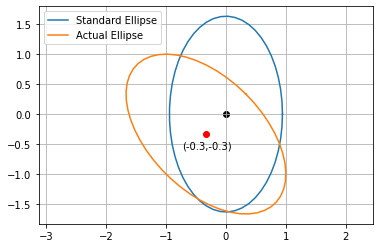
\includegraphics[width=\columnwidth]{ellipse.png}
    \caption{Standard Ellipse centered at origin and Actual Ellipse centered at $(-0.3,-0.3)$.}
    \label{tangent}
\end{figure}
\end{document}
